\chapter{Introducci'on}
% 
% Existen dos tipos de citas bibliograf'icas: usa \verb|\citep{..}| para
% citas en \emph{par'entesis} y \verb|\citet{..}| para citas
% en el \emph{texto}. Por ejemplo, estudios reciente han mostrado nuevos e
% interesantes modelos que se pueden aplicar para reformular teor'ias
% f'isicas~\citep{NewCam97}. Mientras que, el trabajo de \citet{Rofl06} fue
% considerado muy divertido por una significativa fracci'on de la comunidad
% de investigadores. Tambi'en es posible citar a varios trabajos en una sola
% referencia \citep{Lamport86,Knuth84}.



\section{Conformación de proteinas}
\begin{itemize}
 \item proteinas globulares
 \item folding
 \item estados intermedios de plegamiento
 \item IDPs
 \item misfolding + aggregation + amyloid formation
\end{itemize}


The structure-function paradigm claims that a specific function of a protein is determined by its unique and rigid three-dimensional (3D) structure. 
Thus, following its biosynthesis on the ribosome, a protein must fold to a native, defined 3D structure to be functional. 
The primary origin of this structure-function paradigm is the “lock and key” hypothesis formulated in 1894 by Emil Fischer to explain the astonishing specificity of the enzymatic hydrolysis of glucoside multimers by different types
of similar enzymes. For a long period of time, the validity of “lock and key” model and its associated sequence-structure-function paradigm was unquestioned, especially after the crystal structures of proteins started to be solved by X-ray diffraction

Este paradigma se deriva de los primeros avances en el estudio de estructuras de proteinas. Over the past century evidence steadily accumulated that a well-defined structure is the prerequisite of protein function.



Basic biology and biochemistry textbooks that explain biological phenomena at the molecular level exquisitely rely on this notion, the ‘structure–function paradigm’.

Although deviations from this norm were always apparent, they had been invariably neglected or ignored.
Mas adelante en el tiempo se fue encontrando que, además de las estructuras globulares funcionales mas estudiadas, proteins also populate various other states under native, functional conditions, including disordered and partially ordered conformations, and different aggregated assemblies.
Although it was evident from early studies that both soluble and fibrillar forms of proteins could exist (33 ????) , most attention was focused on the soluble states that were found to possess demonstrable biological function.




En el grafico (*** poner grafico de proteostasis que tiene un estado 'nativo' , un estado 'misfolded' y los demas estados de agregacion, etc) se ve que al sintetizarse, 
la proteina naturalmente tiende a ir adquiriendo una conformacion estructural (conjunto de conformaciones mas restringida).
Lo que se fue desarrollando en los ultimos años es que el estado funcional no pertenece(siempre) a una estructura altamente definida sino que puede pertenecer a un conjunto de conformaciones que van desde
estado plegado hasta estados desestructurados, que pueden confundirse con estados totalmente desordenados. 
% fall onto a structural continuum, from tightly folded single domains, to multidomain proteins that might have flexible or disordered regions, to compact but disordered MOLTEN GLOBULES and, finally, to highly extended, heterogeneous unstructured states 
Thus, not just the ordered state but any of the known polypeptide conformations can be the native state of a protein.

Las sintesis de proteínas en el ribosoma puede verse mejor como el punto de inicio para que cada proteina tome una ruta particular a medida que emerge y se acopla al entorno celular. 
Entre las posibles rutas esta la adquisicion de un continuo de estructuras conformacionales funcionales, la adquisicion de una estructura distinta a la funcional(misfolding), y una variedad de estados de agregacion.

% adquiera un continuo de estructuras conformacionales funcionales a medida q emergen y se acoplan al entorno celular.% adoptando la estructura que la caracteriza .

Es por esto que las propiedades conformacionales de una proteína quedan mejor definidas si se declara el conjunto de multiples estados accesibles por sus estructuras.
% A este continuo de conformaciones que pueden adoptar las proteinas individuales, se agregan distintos tipos de estados agregados, conformados a partir de uniones entre proteinas en distintas conformaciones iniciales(conformaciones desestructuradas, intermedios o plegados).
De acuerdo con esta forma de ver, esta accesibilidad estará dada por la estabilidad termodinámica de cada conformacion accesible y la cinética de interconversión entre estas.
Estos requerimientos pueden indicar por ejemplo q ciertos estados altamente estables como puede ser las fibras amiloides no sean estados naturales comunes debido a los requerimientos cinéticos, a pesar de ser termodinamicamente estables.
% De acuerdo con esta forma de describir las posibles conformaciones de las proteinas, the various fates awaiting a polypeptide chain once it has been synthesized in the cell 
% will depend on the kinetics and thermodynamics of the various equilibria between di¡erent possible states.

Las propiedades cinéticas y termodinámicas están dadas por el contexto celular (pH, iones, concentracion de proteinas, presencia de otras moleculas con las que interactúa, etc) y, obviamente, por los posibles cambios que puede tener una proteina,
ya sean mutaciones o modificaciones postraduccionales.
% Las propiedades estructurales de una proteina, descritas de esta forma, pueden modificarse para una proteina a partir de cambios en el contexto(pH, iones, concentracion de proteinas, presencia de otras moleculas con las que interactúa, etc) 
% y, obviamente, también a partir de mutaciones o modificaciones quimicas sobre ésta. 
Esta forma de ver las propiedades estructurales permite ver los origenes de los cambios conformacionales desde el punto de vista de las propiedades fisicoquimicas de las proteinas.
If the stability or cooperativity of the native state of a protein is reduced, for example by a mutation, the population of non-native states will increase.


Es importante destacar, entonces que, for a given polypeptide chain a chosen fate is not a final one, and a choice may be further modulated by environmental pressure. 
Thus, intrinsically unstructured proteins may be forced to fold or misfold via modification of their environment (addition of natural binding partners, changes in properties of solvent and so on), whereas a destabilizing environment may push a natively
folded protein to the misfolding route. Alternatively, the
presence of chaperones may reverse the misfolding route
and effectively dissolve small aggregates




Durante la última década, uno de los mayores cambios en el campo de las proteínas ha sido el reconocimiento de la ubicuidad e importancia de las proteínas intrínsecamente desordenadas. 
% \cite(INTRINSICALLY UNSTRUCTURED PROTEINS AND THEIR FUNCTIONS)
Las proteinas en solucion fall onto a structural continuum, from tightly folded single domains, to multidomain proteins that might have flexible or disordered regions, to compact but disordered MOLTEN GLOBULES and, finally, to highly extended, heterogeneous unstructured states (FIG. 1) 
% This continuum has been interpreted in terms of a ‘PROTEIN TRINITY’ (ordered, molten globule and RANDOM COIL 20 ) or ‘PROTEIN QUARTET ’ 
As the main criterion of a native protein is its ability to perform a biological function, these partially or completely disordered proteins must be regarded as native entities.

% Si bien decimos aca que las proteinas pueden adquirir estructuras correspondientes un ensamble de estructuras accesibles , es posible hacer una clasificación entre proteinas que adoptan estructuras plegadas(con un estado nativo definido por un pequeño conjunto de estructuras) 
% y proteínas intrínsecamente desestructuradas (que adoptan estructuras correspondientes a un gran ensamble continuo de conformaciones). Luego se tratará las conformaciones agregadas de proteínas como una dimensión conformacional distinta.







\subsection{Proteinas globulares}
% En el caso de proteinas altamente estructuradas, la búsqueda de la estructura nativa no es un proceso trivial, y ha promovido la investigación de estructura de proteínas durante muchos años
El proceso mediante el cual una proteína adquiere (rápidamente) 









\subsection{Proteinas intrínsecamente desestructuradas}

Varios reviews en \cite{uversky2010understanding,dyson2005intrinsically}.

The suggestion that the native state of many proteins is intrinsically disordered (or, as originally termed, unstructured) is now integral to our general view of protein structure and function.
Como se dijo en la introduccion, a little more than 10 years ago,however, such challenge to the almost dogmatic ‘structure–function paradigm’ was pure heresy due to the overwhelming evidence that structure determines function.
A decade of steady progress turned skepticism around.
Como parte de estos avances, en los ultimos años se han encontrado gran cantidad de proteinas que adoptan estructuras cuyas conformaciones son total o parcialmente desordenadas(segmentos globulares), soportando esta definicion, formalizada a principios de milenio. 
the transition in paradigm was enforced by scattered experimental observations of disorder in a few dozen proteins. 
% una de las dudas que se tenia era si este estado conformacional existia solo in vitro y en realidad in-vivo lo que ocurria era que el crowding generaba el plegamiento
Evidence added to that obtained by other techniques [mostly NMR and circular dichroism (CD)]..... and the evidence seems overwhelming now that structural disorder also exists in vivo and it is truly the native, functional state of these proteins.


Estas secuencias presentan en solución un conjunto heterogéneo de conformaciones fácilmente maleable por cambios en el medio. 
En lugar del análisis estructural clásico basado en dominios globulares, podemos describir estos conjuntos conformacionales en términos de los promedios y desviaciones estándar de la distancia entre los extremos de la secuencia, el radio hidrodinámico, el contenido en estructura secundaria y otros parámetros (20).

Ten years ago, only predictor of natural disordered regions (PONDR) was available [14]; today, one can use any of about 50 predictors, which are based on several different principles \cite{he2009predicting}.
Como parte de estos ultimos años de investigacion se encontro una gran cantidad de funcionalidades y mecanismos asociados a proteins IDP(ver seccion funciones).
Se desarrollaron tambien bases de datos específicas (ver disprot, y IDEAL: Intrinsically Disordered proteins with Extensive Annotations and Literature. ) y aplicaciones bioinformáticas capaces de identificar el desorden intrínseco (19).

% The identification of many IDPs  enabled the development of sophisticated bioinformatic algorithms for predicting disorder from sequence, which further advanced the field.
The availability of such predictors further advanced the field.
Based on predictions, we know that structural disorder is abundant in all species, and due to its strong correlation with regulatory and signaling functions, its level is significantly higher in eukaryotes than in prokaryotes
Although it has become almost commonplace in the field that structural disorder increases with the complexity of the organism, the highest levels are not witnessed in the most complex metazoan eukaryotes (e.g., in humans), but in single-celled eukar-
yotes that lead a host-changing lifestyle

% TERMINOLOGIA
En un principio se comenzo a definir a este tipo de secuencias como desestructuradas, indicando que prescindian completamente de estructura, aun sabiendo que they have potentially function-related
short- and long-range structural organization, which eventually called upon a change in terminology.
At that time, high-resolution data were rather limited, thus the concept was mostly phrased from the global structural level, which suggested that IDPs fall into coil-like, pre-molten globuletype and molten-globule types
% aca deberia ir algo sobre estudios estructurales que se han hecho
These and many other studies made the term unstructured obsolete. 
% IMPORTANTE
The distinguishing and unifying feature of these proteins – if any – is their inability to fold into a unique and stable tertiary structure
The terms intrinsically unstructured and natively unfolded may be also be suitable for extended random coils and even those that are collapsed, but these terms don't seem to appropriately describe proteins that form transient or
stable secondary structure. The term disorder suffers because of its negative connotation and its possible confusion with a pathological state, yet, on the other hand, disorder can be used for proteins like the molten globule that form substantial secondary structure but that
nevertheless are highly dynamic and non-uniform. For this last reason, herein we will call these proteins “intrinsically disordered” (ID).
By “intrinsic disorder” we mean that the protein exists as a structural ensemble, either at the secondary or at the tertiary level.

% DISORDER vs FLEXIBILITY:
Disorder and flexibility are often used synonymously, but the two terms are quite distinct\cite{radivojac2004protein}. With regard to an ordered protein, flexibility refers to the magnitudes of the excursions of the atoms from their equilibrium positions.
For a disordered region, variation in flexibility refers to differences in the speed of interconversion among the various members of the structural ensemble. A variety of methods have been
used to investigate the flexibilities of disordered regions and proteins, including NMR.


% PROPIEDADES ESTRUCTURALES
A combination of experimental and theoretical studies has clarified how given sequences define specific free energy surfaces that enable folding.
A diferencia de estas superficies energeticas, caracteristicas de las estructuras con plegamiento definido, in some cases the native state of a given peptide or protein may not be structured in a globular form but disordered.

In general, proteins with intrinsically disordered sequences cannot bury sufficient hydrophobic core to fold spontaneously into the highly organized 3D structures that characterize the proteins that are represented in the Protein Data Bank (see the online links
box). In some cases, compact but disordered molten-globule-like states can be formed, or local regions of the sequence can have a propensity to adopt isolated and fluctuating elements of secondary structure (which is equivalent to the ‘pre-molten globule’ proposed by Uversky 2 ). 

Structural disorder can now be studied in great detail by several dozen experimental techniques [21], and the most spectacular advance has been achieved through the application of multidimensional NMR. This approach is often
complemented by other structural techniques, such as small-angle X-ray scattering (SAXS), which is combined with advanced computational data integration based upon molecular dynamics (MD) simulations (Figure 1). These new
approaches [22] enabled the characterization of the full structural ensemble of several dozen IDPs

It is probable that proteins rarely, if ever, behave as true random coils, especially in non-denaturing media: even in their most highly unfolded states, proteins show a propensity to form local elements of secondary structure or hydrophobic clusters






%%% 
% .............

Todas estas propiedades hacen que parezca razonable que este tipo de proteínas este altamente regulada dentro de la célula \cite{gsponer2008tight}.

















\subsection{Misfolding \& Aggregation}

% The sequences of proteins have evolved in such a way that their unique native states can be found very efficiently even in the complex environment inside a living cell. 

contrary to the process of productive protein folding, leading to the appearance of rigid conformation with specific function, the end products of misfolding may have a different appearance. 
The morphology of these end products depends on the particular experimental conditions, and misfolded product may appear as soluble oligomers, amorphous aggregates or amyloid-like fibrils. 
Any of these three species could be cytotoxic, thus giving rise to the development of pathological conditions. 
The reason for such a morphological difference is potentially connected with the diversity of the partially folded intermediates favoring protein self-association. 
In fact, multiple environmental factors, such as point mutations, decrease in pH, increase in temperature, the presence of small organic molecules or metal ions, and other charged molecules, might induce structural rearrangements within a protein molecule, shifting equilirium toward the partially folded conformation(s). As different factors may stabilize slightly different partially folded intermediates, the formation of morphologically
different aggregates is expected.


Como se dijo en las secciones cuando se habló sobre el proceso de plegamiento, las secuencias de proteinas con estructuras plegadas have evolved in such a way that their unique native states 
can be found very efficiently even in the complex environment inside a living cell.

Sin embargo, as the size and complexity of proteins increase, therefore, the folding process becomes more complex. 
Intermediates with only partially formed structures can be populated and have significant lifetimes. 
Under some conditions, then, proteins fail to fold properly or to remain correctly folded; this misfolding can lead to the development of different pathological conditions.
In addition, events that may be termed 'misfolding' may take place during the search for the stable native-like contacts between residues. 
That such complexities are seen even in the benign environment of a dilute solution of a pure protein suggests that they are even more likely to occur in the crowded environment of the cell.

Protein misfolding is a wide-spread phenomenon. Any protein with changes in native structure which affect its normal function is misfolded. 
The terms 'misfolded' and 'aggregated' are not equivalent. Como se verá en las proximas secciones, la habilidad de una proteina formar agregados desestructurados o fibras depende de muchos factores, including protein sequence and environment.
De otra forma, las proteinas que adquieran conformaciones no estructuradas o que se encuentren en estados de plegamiento intermedios semi-estables tendrían una gran tendencia a la agregación, sin embargo esto no es así. 
De hecho, sólo una pequeña fraccion de tales conformaciones tiene tendencia a formar agregados







% **************** AGGREGATION

Proteins might aggregate into ordered(fibrillar amyloids) or amorphous aggregates structures, utilizing relatively short sequence stretches, usually organized in b-sheet-like assemblies. 
These differences in structure also reflect biological differences; amyloid and amorphous beta-sheet aggregates have different chaperone affinities, accumulate in different cellular locations and are degraded by different mechanisms.

La mayoria de las proteínas forma agregados desordenados, caracterizados por la falta de una estructura tridimensional regular(amorfos).
En condiciones fisiologicas, sin embargo, varias proteinas pueden agregarse formando estructuras altamente ordenadas conocidas como fibras amiloides.
Si bien no se van a dar detalles puntuales de la estructura, se sabe que estas diferencias que se ven en la estructura macromolecular son el reflejo de diferencias en las interacciones y estructura a nivel atómico.


De forma gráfica, los equilibrios de agregacion pueden verse en la figura \ref{aggregationDiagram}

\begin{figure}[h!,centered]
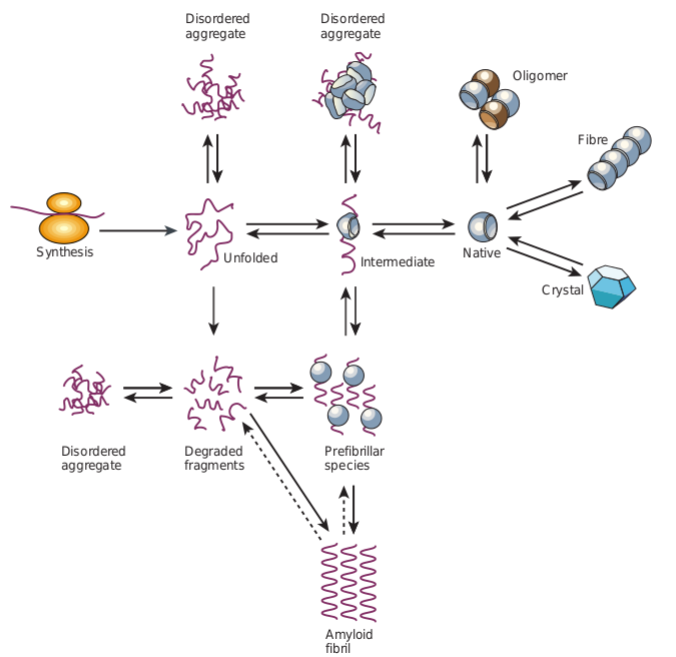
\includegraphics[width=\textwidth]{img/aggregationDiagram.png} 
\caption{Equilibrio de los estados de agregación} \label{aggregationDiagram}
\end{figure}



De la figura puede verse también, que pueden ocurrir distintos procesos de agregación, que resultan en disintas estructuras agregadas, a partir de distintas estructuras adoptadas por las proteinas.

The critical step in the aggregation process is the unfolding of the native structure. 
En la mayoria de las proteinas, excepto las mas pequeñas, el 'unfolding' que ocurre en condiciones fisiologicas no lleva a una estructura totalmente desplegada sino que la proteina adquiere una estructura semi-estable parcialmente collapsada,
donde las interacciones no son las mismas que en el estado nativo estructurado, estas son caracteristicas propias de los intermediarios del plegamiento.
La formacion de estos intermediarios es importante porque generalmente son mucho mas solubles que si se formaran conformaciones altamente desplegadas. 
Esta solubilidad permite alcanzar las concentraciones requeridas para la nucleacion propia de la formacion de amyloids(y de agregados en general????)





% ***********************************************************
% ******* PROPIEDADES DE FORMACION DE AMYLOIDS
% ***********************************************************

Amyloidogenic proteins are quite diverse, with little similarity in sequence and native three-dimensional structure.
Additionally, several proteins and peptides not related to amyloidoses have the potential to form amyloid fibrils in vitro, suggesting that this ability for structural rearrangement and aggregation may be inherent to proteins.
Even though the ability to form amyloid fibrils seems to be generic(is a general property of the polypeptide backbone), the propensity to do so under given circumstances can vary markedly between different sequences(depends enormously on amino acid composition.).

This picture enables us to speculate on the origins of
the amyloid diseases from the point of view of the
physico-chemical properties of the protein molecules. If
the stability or cooperativity of the native state of a
protein is reduced, for example by a mutation, the popu-
lation of non-native states will increase.
This rise will increase the probability of aggregation, as the
concentration of polypeptide chains with at least partial
exposure to the external environment will be greater.
Whether or not aggregation does occur will depend on
the concentration of protein molecules, the intrinsic
propensity for a given sequence to aggregate when
unfolded, and on the rate of the aggregation process. The
fact that formation of ordered amyloid fibrils can be
seeded, like the well-studied processes of crystallization
and gelation, means that once the aggregation process is
initiated it often proceeds very much more rapidly.
In the absence of seeding there can be
long 'lag' phases before aggregation occurs .
This lag can be thought of as arising because the growth
of a fibril cannot occur until a 'nucleus' of a small number
of aggregated molecules is formed. Such a nucleus can be
formed by the local fluctuations in concentration that
occur in solution as a result of random molecular motion.
When such fluctuations result in a local concentration of
molecules above a critical value, the molecules associate
with one other to form a species that is suficiently large
to have intrinsic stability, and hence to grow in size by
interacting with other molecules in the solution. The act
of seeding provides such nuclei to the solution and hence
reduces or abolishes the lag phase







% **********************
% AGREGADOS AMORFOS
% **************************

Amorphous beta-sheet aggregation, is less position-dependent(than amyloid aggregation) and can, in principle, be achieved by any sequence that can adopt an extended conformation, is sufficiently hydrophobic and has no unsatisfied hydrogens or electostatic groups. 
Thus beta-sheet aggregation can be relatively easily predicted by methods that evaluate aggregation by evaluating biophysical parameters over a sequence segment, without the need for considering position-dependent values of these parameters.
















\subsection{Herramientas y mecanismos de proteostasis}
En secciones previas(en la introduccion) se dijo que el espacio de conformaciones accesibles por las proteinas dependia de las estabilidades termodinamicas de los estados y la cinetica de interconversión entre estos. 
Estas propiedades, a su vez, dependen del contexto celular en el que se encuentran(ademas de la secuencia de la proteina en si misma), concentraciones de proteinas, localizacion, interacciones, etc.
El balance correcto entre todas estas condiciones está regulado a traves del proceso de proteostasis.
Proteostasis refers to controlling the concentration, conformation, binding interactions (quaternary structure), and location of individual proteins making up the proteome by readapting the innate biology of the cell, 
often through transcriptional and translational changes.
The protein components of eukaryotic cells face acute and chronic challenges to their integrity. Eukaryotic protein homeostasis, or proteostasis, enables healthy cell and organismal development and aging and protects against disease
Los mecanismos dentro del proceso de proteostasis permiten successful organismal development and aging in the face of constant intrinsic and environmental challenges %previniendo el desarrollo de enfernedades.

La proteostasis es influenciada por todos los mecanismos que controlan los aspectis vistos en las secciones previas..... by the chemistry of protein folding/misfolding and by numerous regulated networks of interacting and competing biological pathways 
that influence protein synthesis, folding, trafficking, disaggregation, and degradation.

La celula posee distintos mecanismos para regular estos procesos .....chaperonas para regular el proceso de folding/misfonding (y tambien de aggregation), 
Nature developed very sophisticated protection mechanisms (chaperones, proteasome, etc.) for the effective regulation of the folding process, y por lo tanto prevenir las peligrosas consecuencias de misfolding. 
In other words, in the cell, any given protein is not acting in the isolation, is never alone and is
constantly "watched" by the protective machinery. This machinery is rather robust and can
tolerate significant loads. Obviously, factors that affect these protective mechanisms will
contribute to the probability of disease development


-Cells possess a complex proteostasis network (PN) to ensure protein homeostasis.
-Aggregates permanently engage molecular chaperones and other PN components.
-The PN is challenged by chronic stress in protein-aggregation diseases and aging.
-Overtaxing the PN drives a vicious cycle of disease progression with eventual proteostasis collapse.



Las diferencias estructurales vistas entre los distintos estados de agregación tambien se ven reflejada en diferencias biológicas 
Whereas misfolded and aggregated proteins are found in perinuclear locations and are generally degraded by the 
proteasomal system, amyloids preferentially accumulate in perivacuolar inclusions, where they are degraded by the autophagosome.
% This segregation directly results from a differential recognition by the protein quality control system. 
Esta segregación resulta en un tratamiento distinto por parte de los mecanismos encargados de la proteostasis.
A reduced affinity of amyloids for the protein quality control system is probably also at the root of their higher toxicity 11 as artificial overexpression of chaperones
usually leads to decreased toxicity and removal of amyloids from he cell.
Contrary to amorphous aggregates, amyloid structures can fulfill biological functions, and functional amyloids are found in organisms from prokaryotes to humans \cite{fowler2007functional}.





% PREVENCION DE AGREGACION EN FOLDED PROTEINS
the normal folding process may pass through
partially folded states on the route to the fully native state,
but the aggregation of these species will be minimized by
the presence of molecular chaperones. In addition, if the
protein is able to fold rapidly, any partially folded species
will have a short lifetime, reducing the probability of inter-
molecular interactions occurring. Moreover, once folded,
the native state is generally a highly compact structure
that conceals the polypeptide main chain within its
interior. Such a state is protected from aggregation except
through the interactions of surface side chains (as is the
case, for example, in protein crystals) and is unable to
form the strong intermolecular hydrogen bonds associated
with the polypeptide backbone. Provided that the native
state is maintained under conditions where it remains
folded, aggregation to amyloid fibrils will be resisted by
the kinetic barrier associated with unfolding, even if the
aggregated state is thermodynamically more stable.
Importantly, the cooperative nature of protein structures
means that virtually none of the polypeptide chain in indi-
vidual molecules is locally unfolded, and that virtually no
molecules in an ensemble are globally unfolded, even
though native proteins are only marginally stable relative
to denatured ones under normal physiological conditions


% ACA EXPLICO POR QUE LAS IDPs NO TIENEN TANTA TENDENCIA A FORMAR AGREGADOS
In contrast to the globular proteins, which have to unfold prior to aggregation (Jahn and Radford, 2005), IDPs are always ready for intermolecular interactions. 
An unbound fragment of an IDP possesses a strong ability to interact, and therefore can bind either to natural partners forming native complexes or to similar molecules forming various aggregates. 
This raises the question of why IDPs do not always form aggregates in the norm. One of the potential answers is the fact that inside the cell, the IDPs typically form complexes with natural partners.
Los mecanismos de proteccion (chaperonas, proteasoma, etc) tienen una gran capacidad para mantener la solubilidad de proteinas.
Además, based on the analysis of the IDP amino acid composition, it would be clearly a mistake to assume that an averaged IDP possesses higher propensity towards aggregation than an averaged ordered
protein. In fact, many IDPs contain large number of charged and polar residues. In addition to the hydrophobic interactions, the net charge is one of the major factors determining aggregation behavior of a protein.













\section{Características funcionales}
Breve historia estructura-función, motivos secuenciales, funcionalidad en proteinas IDPs


This means that the structure-function paradigm, which emphasizes that ordered 3D structures represent an indispensable prerequisite to effective protein functioning, should be redefined to include intrinsically unstructured proteins [159]. According to this redefined paradigm, native proteins (or their functional regions) can exist in any of the known conformational states, ordered, molten globule, premolten globule and coil. Function can arise from any of these conformations
and transitions between them. Thus, not just the ordered state but any of the known polypeptide conformations can be the native state of a protein.




% FUNCIONALIDAD EN IDPs
The most important question of the field, therefore, is the physiological function and functional mode of IDPs/IDRs.
It is now clear that structural disorder provides multiple functional advantages\cite{gunasekaran2003extended,dyson2005intrinsically},
and IDP functions either directly stem from their disorder (entropic chains) or from molecular recognition, when they undergo induced folding (disorder-to-order transition) upon binding to a partner molecule
The functional role of structural disorder from a biological process view addresses what type of cellular functions benefit most from the lack of a stable structure. This
question was addressed in several large bioinformatics studies. As a result, IDPs are generally thought to be involved in processes of signaling and regulation, and in depth correlation analysis [52] of 710 Swiss-Prot functional keywords suggested significant positive correlation with 238 functions and negative correlation with 302 functions (Table 2). Most of the functions that correlate with the
presence of long disordered regions are related to regulation via transcription and translation, whereas functions
that correlate with the lack of disorder are dominated by
enzymatic catalysis.

Algunas propiedades interesantes de las proteinas IDPs se revelan a partir de estudios a nivel de proteoma y sistema.
As suggested, IDPs/IDRs often function by binding accompanied by induced folding (molecular recognition) [6–8] mediated by SLiMs/ELMs, and in several recent
works it has been shown that the functional and evolutionary agility of IDPs can be ascribed to the inclusion or exclusion of such motifs in RNA maturation; that is, by alternative splicing, alternative promoter usage, and RNA
editing, the alternative isoforms thus generated promote the functional diversification of the proteome
This
mechanism can result in a change in diverse functional attributes, such as subcellular localization, protein–protein interaction, phase transitions and even opposing (dominant negative) function, as also demonstrated by
studying tissue-specific forms of alternative splicing. These protein isoforms tend to occupy central positions in interaction networks and their pattern of interaction partners tend to significantly differ [63]; that is, structural disorder
and encoded motifs have a strong potential to define and redefine wiring of cellular signaling pathways.













\section{Arquitectura de proteínas}
dominios funcionales, proteinas multidominio, linkers 


% Many cellular processes involve proteins with multiple domains.
Many eukaryotic proteins are modular — that is,
they contain independently folded globular domains
that are separated by flexible linker regions. 

The modular nature of proteins has many advantages,
providing increased stability and new cooperative functions.
Other advantages include the protection of intermediates within
inter-domain clefts that may otherwise be unstable in aqueous
environments and the fixed stoichiometric ratio of enzymatic
activity necessary for a sequential set of reactions


Protein domains can be defined as segmented por-
tions of a polypeptide sequence that assume stable
three-dimensional structure. 6 Such recurring protein
motifs are significant because it is increasingly recog-
nized that there are only a limited number of domain
families in nature.

These domains are duplicated and
combined in different ways to form the set of proteins
in genomes. 10 The importance of domains is further
exemplified by the fact that multidomain proteins
play a major role in many cellular processes.

Although a consensus in detail is still lacking, various
effective criteria have been proposed to detect and
define protein domains. These criteria rely mainly on
the existence of local structural compactness arising
from beta-sheets or hydrophobic cores. 11,12 Based on
such compactness, computational algorithms to detect
structural domains have been proposed








\subsection{Secuencias linker naturales}
Estructura - Composición -  Estudios sobre linkers naturales
% Algunos linkers en la naturaleza se caracterizan por poseer estructuras rígidas que permiten mantener a los dominios funcionales a una distancia mínima(por lo cual se conocen como molecular rulers).


Linker
sequences vary greatly in length and composition, but
many are rich in polar, uncharged amino acids (such as
Ser, Thr, Gln and Asn), in the small residues Ala and Gly,
and in Pro residues. Many of these residues tend to bias
the polypeptide chain towards the polyproline-II region
of the RAMACHANDRAN PLOT 27,28 .This means that such
linkers, although flexible, have a propensity to be highly
extended. Compositionally biased linker sequences of
significant length are found mainly in eukaryotic pro-
teins 1,29 , but short linker sequences of similar composi-
tion, known as Q-linkers, are also found in a number of
bacterial regulatory proteins 30 .
In the absence of their targets, modular proteins
often behave as ‘beads on a flexible string’, where the
function of the linker is, primarily, to enable a relatively
unhindered spatial search by the attached domains 31 .
However, binding can induce structure formation in
linkers, which can have significant functional conse-
quences. For example, the sequence-specific binding of
CYS HIS ZINC-FINGER PROTEINS to DNA causes the linker to
fold, cap and thereby stabilize the preceding helix in the
protein, and to orientate the next zinc finger correctly
for binding in the major groove of DNA



\subsection{Ingeniería de proteínas}
Objetivos, fundamentos, origen, creacion de proteinas multidominio



\subsubsection{Diseño de linkers artificiales}
Metodos y herramientas disponibles




